\documentclass[crop,tikz]{standalone}

\usepackage{pgfplots}
\tikzset{>=latex}
\usepgfplotslibrary{colormaps}

\begin{document}
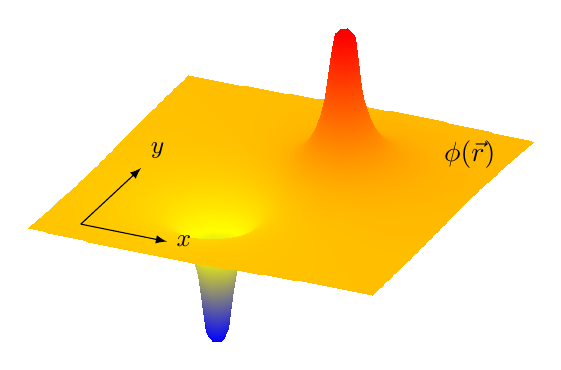
\begin{tikzpicture}
  \begin{axis}[
    width=8cm,
    height=8cm,
    domain=-4:4,
    shader=interp,
    colormap/hot,
    point meta min=-4,
    point meta max=4,
    hide axis,
    zmin=-4, zmax=4,
    clip=false,
    declare function = { f(\x,\y) = - 1/sqrt((\x+1)^2 + (\y+1)^2) + 1/sqrt((\x-1)^2 + (\y-1)^2); },
    ]
    \addplot3[
       restrict z to domain* = -4:4,
       surf,
       samples=70,
    ]{ f(x,y) };
    \node at (axis cs: 3, 3, 0) { $\phi(\vec{r})$ };
    \coordinate (O) at (axis cs: -3, -3.5, 0); % origin
    \draw[->] (O) -- (axis cs: -1, -3.5, 0) node[right] { \small $x$ };
    \draw[->] (O) -- (axis cs: -3, -0.5, 0) node[above right] { \small $y$ };
  \end{axis}
\end{tikzpicture}
\end{document}
